\section[Introduction]{Introduction and Problem Analysis}

\subsection{Background and Task}

A river flood changes the land surface within hours. Emergency managers then have to decide where water now stands that was dry before, how many people and facilities this water reaches, and how relief can still get through a road network that the same water has cut. Synthetic aperture radar (SAR) sees open water through cloud and rain because a smooth water surface reflects the radar pulse away from the sensor and appears dark. Optical imagery taken before the event shows what the land looked like: permanent rivers and ponds, cropland, trees, buildings. The task is a chain of five models built on these two sources.

Problem~1 asks for preprocessing and a recognizer of flood-inundated area on the official Attachment~1 (1000 triplets of pre-flood optical tile, post-flood GF-3 SAR tile and label), evaluated on independent samples with pixel accuracy, the error of newly inundated area, the relative area error and spatial overlap, plus an analysis of false positives (FP) and false negatives (FN) by land cover and of the factors behind area error. Problem~2 asks for a fused, more accurate model whose primary goal is a small area error, and for a four-level intensity grading (general, relatively strong, strong, extremely strong) with explicit area or proportion thresholds and an analysis of how area errors move the grades. Problem~3 transfers the model to the flood around 6 July 2026 in Hengzhou City, Guangxi, and asks for pre-existing water, newly inundated area, net increase, proportion and a map. Problem~4 asks for a regional assessment on self-chosen units with newly inundated area, proportion and intensity as core indicators and with the exposure of people and critical facilities. Problem~5 asks for one rescue optimization fed directly by the image and assessment results, and for a letter to the local emergency authority.

Fig.~\ref{fig:scenario} fixes the scene behind these five questions. A permanent channel runs along the valley floor, a road follows the terrace above it, and the settlements stand on ground that is normally dry. During the event the floor is covered by new water, the road is cut where it dips into the flood, and a terrace settlement can be reached only by boat.

\begin{figure}[!ht]
  \centering
  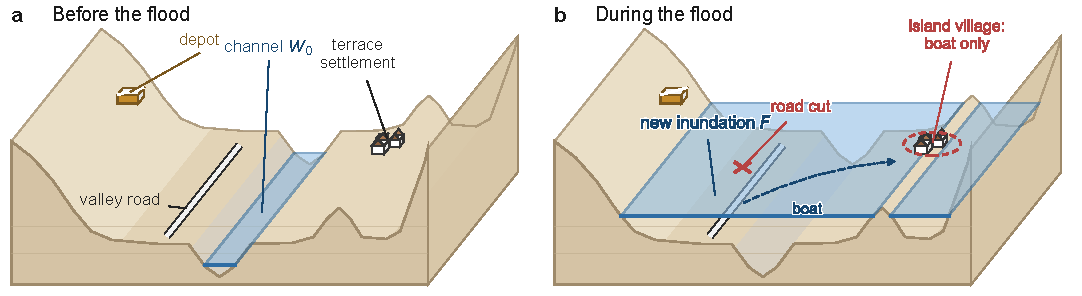
\includegraphics[width=0.90\textwidth,keepaspectratio]{../figures/fig_scenario.pdf}
  \caption{Schematic flood-inundation scenario}
  \label{fig:scenario}
\end{figure}

\subsection{One Definition Shared by All Five Problems}

One chain, one quantity. Because the five problems pass one object from link to link, the definition is fixed here once. We use
\begin{equation}
F=W_1\setminus W_0,\qquad A_{new}=\sum_{p\in F}a_p,\qquad A_{net}=\sum_{p\in W_1}a_p-\sum_{p\in W_0}a_p,\qquad \rho=\frac{A_{new}}{A_{reg}},
\label{eq:def_F}
\end{equation}
where $W_0$ is the water before the flood, $W_1$ the water at the observation time, $a_p$ the true ground area of pixel $p$ and $A_{reg}$ the area of the region or unit. ``Newly inundated area'' is the set $F$ itself; the net increase $A_{net}$ subtracts water that disappeared and can never exceed $A_{new}$ (Section~\ref{sec:data_def}). Two traps follow directly from \eqref{eq:def_F}: counting all post-flood water as new inundation, and reporting the net increase as the new area. Both are avoided by construction.

\subsection{Modeling Route}

Five objects travel along the chain, and Fig.~\ref{fig:roadmap} draws the hand-offs; the arrow labels are those objects, nothing else. From Problem~1 come the baseline recognizer, its FP/FN hotspots by land cover and the hard tiles. A fused model with an area-preserving threshold $\tau_A$ and the grade thresholds $\theta_g$ is what Problem~2 makes of them. Applied unchanged to Sentinel-1 imagery of Hengzhou, that model yields the raster $F$ (Problem~3). Overlaid with population, land cover, roads and facility proxies, $F$ ranks the assessment units of Problem~4; that raster then deletes flooded roads and depots in Problem~5, where the flooded population and index of Problem~4 become demand and priority of a depot-activation and allocation model.

\begin{figure}[!ht]
  \centering
  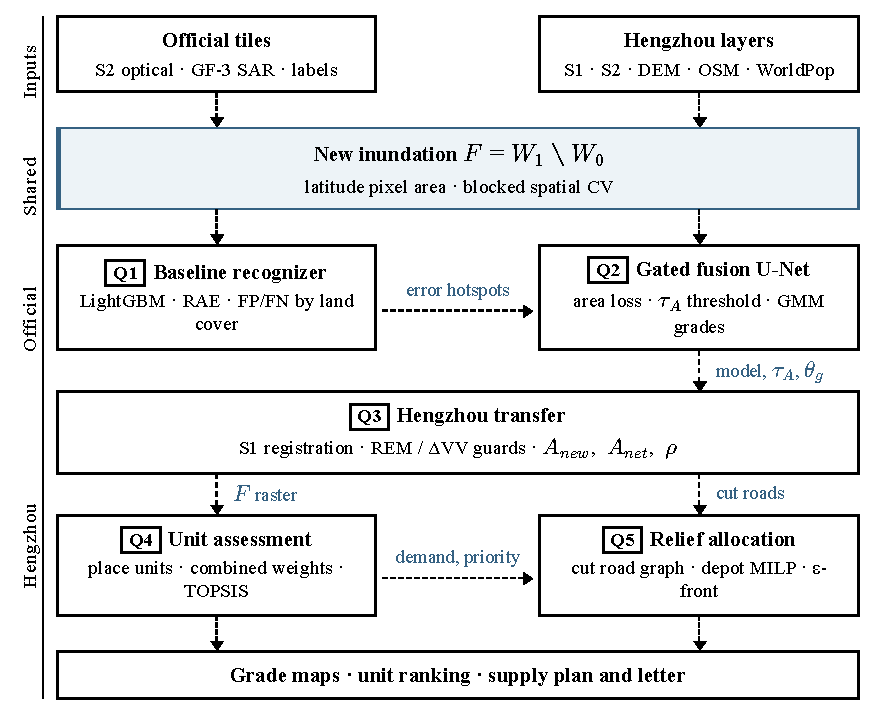
\includegraphics[width=0.82\textwidth,keepaspectratio]{../figures/fig_roadmap.pdf}
  \caption{Technical route of the five-problem chain}
  \label{fig:roadmap}
\end{figure}

Where the two data worlds meet is also drawn in Fig.~\ref{fig:roadmap}. Official tiles occupy the upper half: labels exist there, and every metric can be computed on held-out tiles. The lower half holds only self-collected Hengzhou layers, where no labels exist; there the model output is filtered by physical guards and checked by label-free consistency tests. Training never mixes the two datasets, and exactly three objects cross the boundary: the frozen network weights, the calibration $\tau_A$ and the thresholds $\theta_g$. That separation keeps the Hengzhou numbers of Problems~3--5 traceable to a model whose accuracy was measured on Attachment~1, never tuned towards it.

\subsection{Related Work and What This Paper Adds}

Threshold methods on SAR backscatter remain the operational standard. The split-based rule of Martinis et al.~\cite{martinis2009splitbased} selects bimodal sub-blocks before Otsu's threshold, and automated Sentinel-1 chains add change detection against a reference scene~\cite{twele2016sentinel1}. Deep segmentation networks of the U-Net family~\cite{ronneberger2015unet} trained on labeled Sentinel-1 chips~\cite{bonafilia2020sen1floods11} improve pixel accuracy, but they are usually judged by IoU, not by the area that a disaster report quotes. Terrain descriptors such as the height above the nearest drainage~\cite{nobre2011hand} are commonly used to exclude implausible water on slopes. Relief logistics after a disaster is a facility-location and allocation problem~\cite{balcik2008facility}.

Each choice below answers a gap documented in the cited work, and the first gap is what the recognizer should learn. Testing the official labels on all 65.5 million valid pixels showed that they encode new inundation; the recognizer learns $F$ directly, while Problem~3 still enforces $F\cap W_0=\emptyset$ with an independent $W_0$. Training then targets the area itself. An isotonic probability map followed by an area-preserving threshold makes the mask area equal to the calibrated expected area, and split-conformal intervals attach an error band to every tile. Grade boundaries sit where adjacent components of a Gaussian mixture on the logit flood share are equally likely, with block-bootstrap intervals; a grade becomes a probability vector and not a label alone. The same raster enters the relief model twice, through the cut road graph and through the demand and priority of each unit, and the worth of the second satellite pass becomes the change of the optimal unmet share\cite{deepseek2026,qwen2026,doubao2026}.
